\newpage
\section{Concatenation}
\begin{enumerate}
	\item[1)]
		\begin{lstlisting}[caption={Concatenation kode},label={lst:ConcatenationCode}][htpb]
	library ieee;
	use ieee.Std_logic_1164.all;
	
	entity shift_div is
	port (a : in std_logic_vector(7 downto 0);
	a_shl,a_shr,a_ror: out std_logic_vector(7 downto 0));
	end shift_div; 
	
	architecture dataflow of shift_div is
	
	begin 
	a_shl <= a(6 downto 0) & '0';
	
	a_shr <= "00" & a(7 downto 2);
	
	a_ror <= a(2 downto 0) & a(7 downto 3);
	
	end dataflow ;

		\end{lstlisting}
	\item[2)]
Vi kan se på figur \ref{fig:concatenationRTL} fra RTL-viewer, at der ikke er nogen logiske elementer i kodestykket:
	\begin{figure}[H]
		\centering
		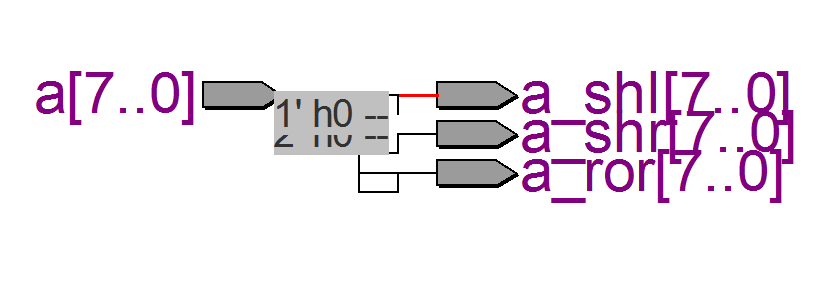
\includegraphics[scale=0.5]{pictures/Oevelse3/Concatenation_RTL.png}
		\caption{Concatenation RTL}
		\label{fig:concatenationRTL}
	\end{figure}

	
	\item[3)]
Vi overfører programmet til DE2-boardet. Inputtet a sættes som SW[7:0], output a-shl sættes til LEDR[7:0], a-shr sættes til LEDR[17:10] og a-ror sættes til LEDG[7:0]. Dette kan ses på figur \ref{fig:concatenation_DE2board}.

	\begin{figure}[H]
		\centering
		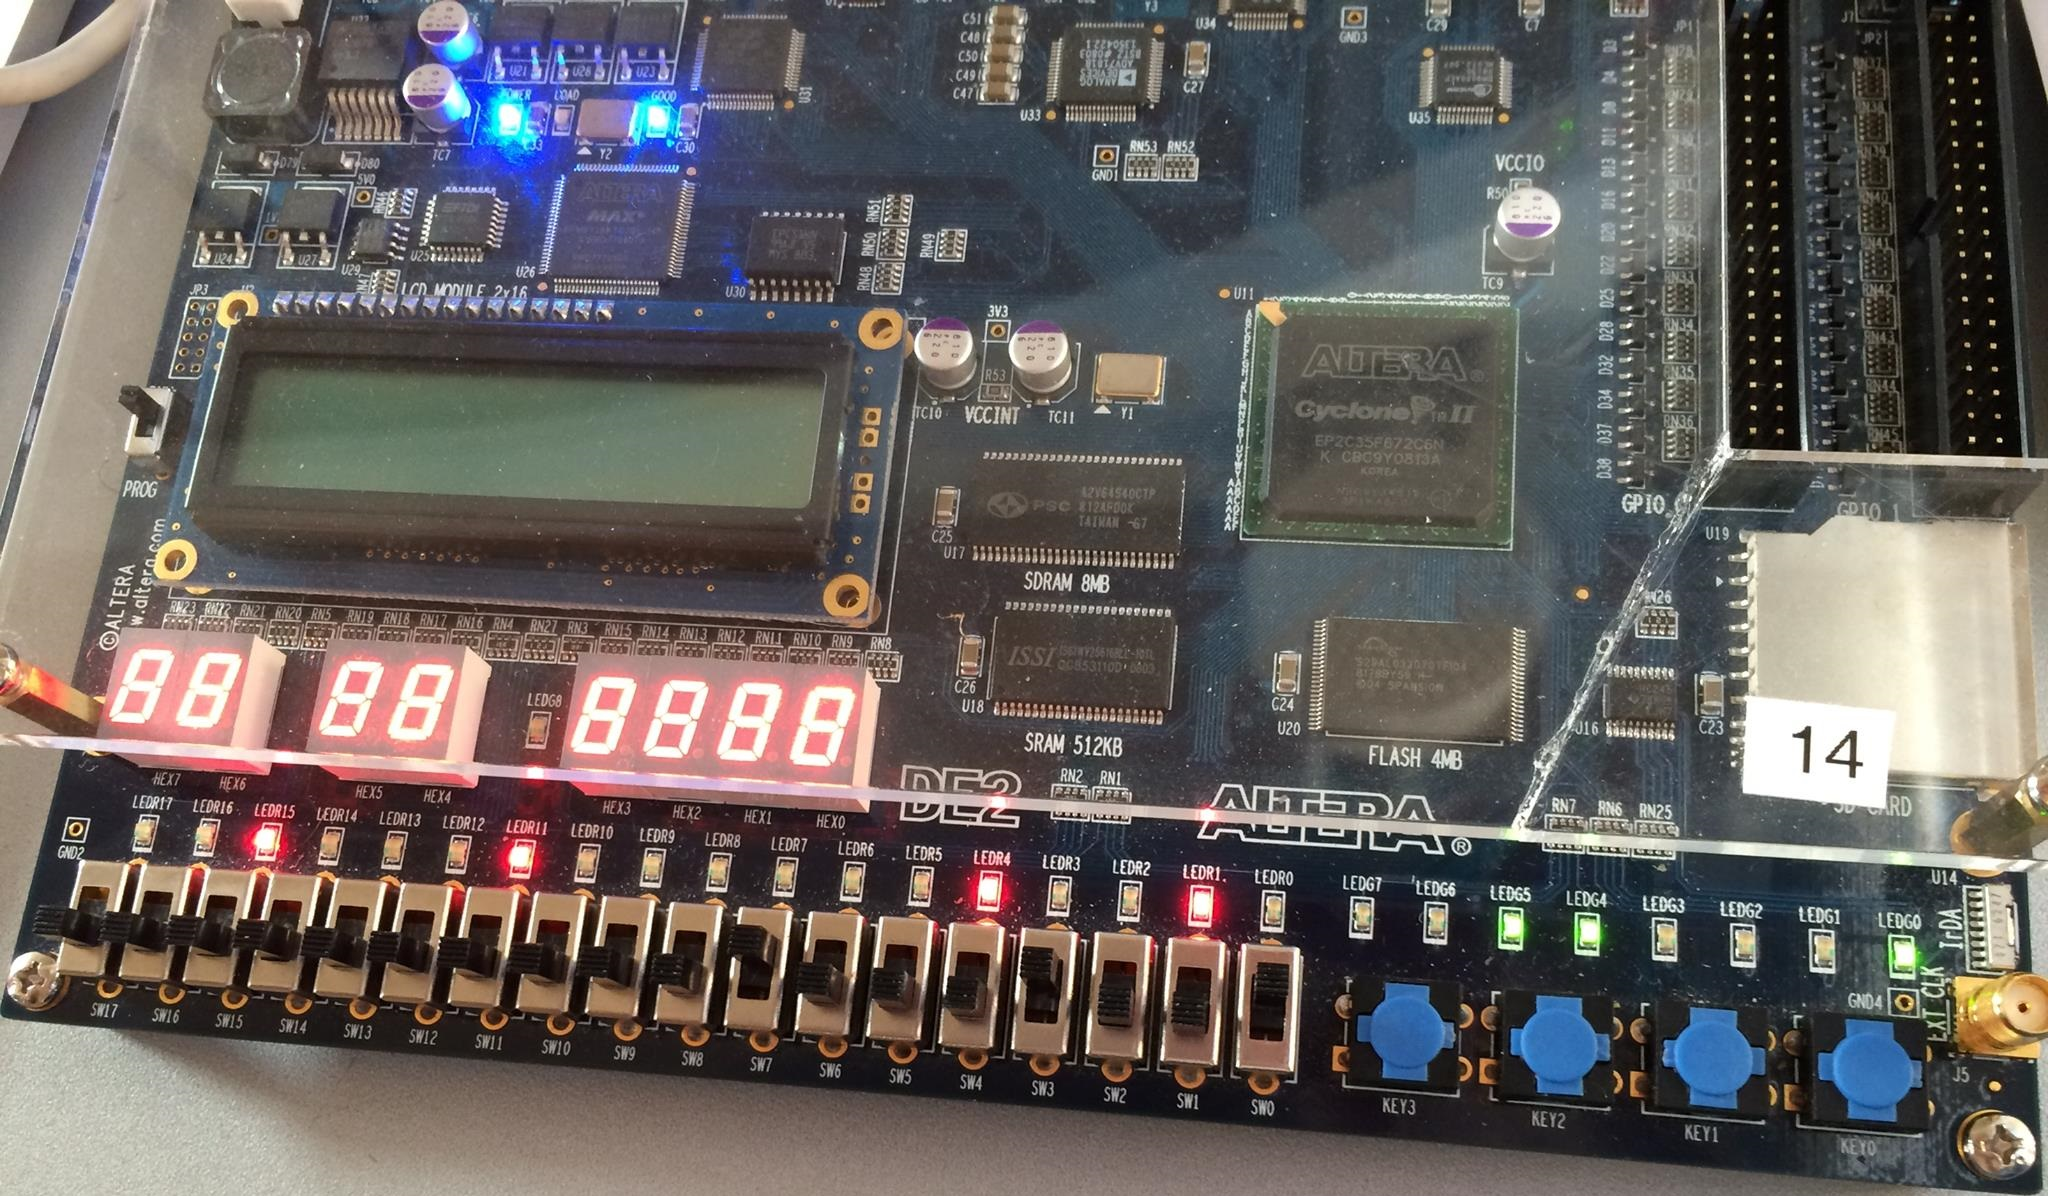
\includegraphics[scale=0.23]{pictures/Oevelse3/Concatenation_DE2board.jpg}
		\caption{Concatenation på DE2-board}
		\label{fig:concatenation_DE2board}
	\end{figure}

\end{enumerate}
\pagebreak